\documentclass[twocolumn]{article}
\usepackage[margin=1in]{geometry}
\usepackage[utf8]{inputenc}
\usepackage{hyperref}
\usepackage{amsmath}
\usepackage{enumitem}
\usepackage[justification=centering]{subfig}
\usepackage{numprint}
\usepackage{booktabs}
\usepackage{multirow}
\usepackage{wrapfig}
\usepackage{float}
\usepackage{relsize}
\usepackage{tikz}
\usepackage{pgfplots}
\usepackage{pgfplotstable}
\pgfplotsset{compat=newest}
\usepgfplotslibrary{colorbrewer}

\title{ALiEN: the Sum Game}
\author{Timothee Mickus}
\date{August 2021}

\begin{document}

\maketitle

\section{Introduction}

Emergent communication studies generally focus on games: setups involving agents that must interact through communication in order to solve a task.
Our focus here is on the ``sum game''.
The first agent (the ``sender") sees two integers $a$ and $b$ between 0 and $N$ included and produces a message.
The second agent (the ``receiver") is shown this message and must output the sum $a+b$.

Multiple approaches to implement this game can be devised.
Two seem to us particularly relevant.
The first consists in casting this game as a categorization problem: the receiver must select one of $2N+1$ potential targets, given the sender's message.
The second consists in considering the numerical aspect of the game: the receiver must output some scalar value corresponding to the sum $a+b$.
While the former approach suggests to tackle this game using classification tools, e.g., using a cross-entropy loss; the latter suggests to employ scalar regression techniques, e.g., using a mean-squared error loss.
The angle we take here consists in comparing these two approaches, and see whether they impact the emergent communication protocol between the two agents.

%The rest of this report is structured as follows: we set our baseline expectations in Section~\ref{sec:baselines}. 
%We focus more narrowly on our experimental methodology in Section~\ref{sec:experiment}, and detail the results we observe in Section~\ref{sec:results}.
%We conclude with an in-depth manual analysis of the emergent language in Section~\ref{sec:analysis}.

\section{Experimental design} \label{sec:experiment}

%We intend to compare a regression-based implementation of the game to a discrimination-based implementation of the game. 

\subsection{Model implementation} \label{sec:experiment:models}

We design our two types of models to be as similar as possible. 
They are composed of two agents each: one sender, which uses an input pair embedding $E(\langle a,b \rangle)$ to prime a {\sc rnn} and produce a message, and one receiver, which reads the sender's message using a {\sc rnn} and derives a prediction from the final hidden state.

The sole difference between the two types of model is how the final prediction is derived, and the loss function used to train the models.
In the categorization approach, the final hidden state is linearly transformed into a distribution over all $2N + 1$ possible answers; the entire model is then trained to minimize cross entropy.
In the regression approach, the final hidden state is transformed into a scalar value $s$ mapped onto the interval $\left[0~; ~2N \right]$ using a scaled sigmoid function $2N\cdot\sigma(s)$; the entire model is then trained to minimize the squared error. 

\subsection{Data} \label{sec:experiment:data}

Throughout our experiments, we use $N=63$; i.e., all integers $\langle a,b \rangle$ are comprised between 0 and 63 included and their sum $s$ is between 0 and 126. 
This corresponds to $64^2=4096$ possible pairs $\langle a,b \rangle$.
We randomly split all possible pairs $\langle a,b \rangle$ in three groups. 80\% (3276 pairs) are used for training models, 10\% (410 pairs) are used for selecting hyperparameters, and 10\% (410 pairs) are used to further test the model's ability to generalize.
All models are trained and tested and the same random splits, to ensure our experiments are comparable.

\subsection{Hyperparameter space} \label{sec:experiment:hparams}

We consider four categories of hyperparameters.

\vspace*{-0.5em}
\paragraph{Learning mechanism:} 
\begin{enumerate}[label=(\roman*)]
    \vspace*{-0.5em}
    \itemsep-0.25em 
    \item what learning rate to use
    \item \label{it:hp:mechanism} whether gradient is propagated with Gumbel Softmax or {\sc reinforce}
    \item \label{it:hp:temp} what initial temperature to apply to the sender's distribution over the vocabulary (if using a Gumbel Softmax)
    \item \label{it:hp:entropy} what coefficient to apply for the entropy penalty (if using {\sc reinforce})
\end{enumerate}

\vspace*{-0.5em}
\paragraph{Data handling:}
\begin{enumerate}[resume*]
    \vspace*{-0.5em}
    \itemsep-0.25em 
    \item \label{it:hp:batch} how many examples to group per batch
    \item \label{it:hp:avg} whether to average the loss over all examples in a batch
    \item \label{it:hp:ipt} whether to represent inputs with one-hots or binary expansions
\end{enumerate}

Hyperparameter \ref{it:hp:ipt} controls how pairs are presented to the sender.
When using one-hot vectors, we represent an integer $i$ as a vector with $N+1$ components, all of which are set to 0, except for the $i$\textsuperscript{th} component, which is set to 1. 
Binary expansion vectors components correspond to the 0-padded binary expansion of the integer: for example, 25 would be represented with the vector $\langle 0, 0, 1, 1, 0, 0, 1\rangle$, corresponding to its binary notation, 11001, preceded by as many 0 as necessary to encode all numbers in our dataset.\footnote{
    This input format may prove useful in that it limits the number of weights used to represent items and encodes the structure of the input space more explicitly.
}
Pairs of integers are represented by concatenating the two integer representations; pair embeddings are then fed to the sender's {\sc rnn}.

\vspace*{-0.5em}
\paragraph{Model architecture:}
\begin{enumerate}[resume*]
    \vspace*{-0.5em}
    \itemsep-0.25em 
    \item whether to use a {\sc rnn}, {\sc gru} or {\sc lstm}
    \item the dimension of embeddings
    \item the dimension of hidden representations
\end{enumerate}

\vspace*{-0.5em}
\paragraph{Symbolic channel:}
\begin{enumerate}[resume*]
    \vspace*{-0.5em}
    \itemsep-0.25em 
    \item how many distinct symbols to use; i.e., what size of vocabulary to use
    \item \label{it:hp:cl} whether or not to use a curriculum mechanism
    \item \label{it:hp:cl-upd} how often length should be increased
    \item \label{it:hp:cl-len} how many epochs the curriculum should span
\end{enumerate}

We call `curriculum' the following mechanism: instead of using the maximum default length for messages, we set the maximum length to 1 before training begins.
We then increase this maximum length at specific epochs during the training process.
Hyperparameter \ref{it:hp:cl-len} controls the total length of this curriculum, whereas hyperparameter \ref{it:hp:cl-upd} controls how many such increases there are.
Given these hyperparameters, we space these length increments evenly throughout the full duration of the curriculum.\footnote{
    Such a curriculum can in principle prove helpful to the agents.
    Exploring a more limited action space is easier for the sender.
    As messages cannot be too complex, the receiver must also adopt a policy that covers the most general cases.
    Whenever the maximum length is increased, agents can build on their previous language to reach higher accuracy.
}

Hyperparameters do not include maximum message length, which we set to 8 in all experiments, for simplicity.
Also note that the interaction between hyperparameters.
Temperature \ref{it:hp:temp} and entropy \ref{it:hp:entropy} are never in effect jointly, and depend on the gradient propagation mechanism \ref{it:hp:mechanism}; likewise, if the batch size \ref{it:hp:batch} is set to 1, then loss averaging \ref{it:hp:avg} has no effect; lastly, curriculum updates \ref{it:hp:cl-upd} and duration \ref{it:hp:cl-len} depend on a curriculum being set \ref{it:hp:cl}.

\subsection{Selecting hyperparameters} \label{sec:experiment:bayes-opt}

Hyperparameter choices are likely to impact regression game differently from categorization games. %, and therefore using the same hyperparameter configuration for both models is to be avoided.
We therefore require a principled way of selecting hyperparameters. %; for instance, using a grid search or random search approach.
Given the large search space we consider (cf. Subsection~\ref{sec:experiment:hparams}), a grid search would be inefficient.
%Moreover, we wish to take into account that some parameters are interrelated, and therefore a random search approach may not be optimal.
Instead we opt for Bayesian Optimization: we iteratively select hyperparameters that are the most likely to improve some objective value over the current optimum.
The probability of yielding an improvement given a configuration of hyperparameters is updated after each iteration using Bayes' theorem.

We perform 100 iterations in total.
The first 10 iterations are purely random samples of hyperparameter configurations, from which we construct a prior distribution to bootstrap the selection process. 
We use accuracy on a development set as the objective value to optimize.
For each configuration of hyperparameters sampled, we train 3 different models for up to 100 epochs, compute the maximum accuracy they reach on the development set and return the average.%\footnote{
%    This average is motivated by the fact that different runs with the same hyperparameter configuration can in practice bring about very different results.
%}

This methodology is computationally costly. %\footnote{
%    Given the 2 types of models, the 100 hyperparameter configuration sampling, and the 3 runs per configuration, we train 600 models in total.
%}
To limit the time required by each experiment, we implement two mechanisms.
First, we stop early any run that has not improved in accuracy over 10 epochs.
Second, we save the model that performs best on development data at any point during the experiment, and consider only this optimal model in our analyses.
These two mechanisms may impact results: configurations could yield higher performances if we used a longer patience or no early-stopping; likewise, we may end up selecting a model that happens to perform well on the development set.

\section{Results \& Analysis} \label{sec:results}

\begin{table}%{l}{0.6\textwidth}
    \centering
    \smaller
    \begin{tabular}{l r r}
    \toprule
        \textbf{Hyperparameter} & \textbf{Regression} & \textbf{Categorization} \\
    \midrule
        Learning rate & 0.0015 & 0.00025 \\
        Mechanism & {\sc gs} & {\sc gs} \\
        Temperature & 10 & $1.26\cdot10^{-5}$\\
        Entropy coefficient & {\it\smaller (1.0)} & {\it\smaller (0.7)} \\
    \midrule
        Input format & Binary & Binary \\
        Batch size & 2 & 256 \\
        Average over batch & No & Yes\\
    \midrule
        Cell architecture & {\sc gru} & {\sc gru} \\
        Embeddings dim. & 16 & 1024\\
        Hidden dim. & 16 & 1024 \\
    \midrule
        Vocabulary size & 13 & 28 \\
        Curriculum & No & No \\
        C. updates & {\it\smaller (5)} & {\it\smaller (3)} \\
        C. duration & {\it\smaller (28)} & {\it\smaller (31)} \\
    \bottomrule
    \end{tabular}
    \caption{Hyperparmaters for best models}
    \label{tab:hparams-best}
\end{table}

We begin by focusing on the hyperparameters corresponding to the best models, shown in Table~\ref{tab:hparams-best}. 
Hyperparameters that have no effect are displayed between parentheses. 
Some parallels between regression and categorization models exist: both use a {\sc gru}-based architecture, binary expansion vectors, Gumbel-Softmax and no curriculum. 

All other hyperparameters are in stark contrast. 
The regression model employs a lightweight architecture, with comparatively few neurons, whereas the categorization model uses the largest available size.
The regression model uses small batches, while the categorization model uses large batches and averages the loss over all items.
The initial temperature of the Gumbel-Softmax are 6 orders of magnitude apart.
This disparity shows how crucial the hyperparameter selection process is.

\begin{table}%{l}{0.5\textwidth}
    \centering
    \npdecimalsign{.}
    \nprounddigits{3}
    \subfloat[\label{tab:auto:reg}Regression-based game]{
        \begin{tabular}{l n{1}{3} n{1}{3} n{1}{3}}
        \toprule
            & {{\textbf{Train}}} & {{\textbf{Dev}}} & {{\textbf{Test}}} \\ 
        \midrule    
            {\sc mse}  & 0.26009419560432434 & 0.259131520986557 & 0.2690547704696655 \\
            Acc. & 0.711843729019165 & 0.7414634227752686 & 0.7341463565826416 \\ 
        \bottomrule    
        \end{tabular}
    }

    \subfloat[\label{tab:auto:cat}Categorization-based game]{
        \begin{tabular}{l n{1}{3} n{1}{3} n{1}{3}}
        \toprule
            & {{\textbf{Train}}} & {{\textbf{Dev}}} & {{\textbf{Test}}} \\ 
        \midrule    
            {\sc xent} & 2.71825909614563 & 2.750857353210449 & 2.7228848934173584  \\
            Acc. & 0.1913919448852539  & 0.19512194395065308 & 0.1634146273136139  \\  
        \bottomrule
        \end{tabular}
    }
    \caption{\label{tab:auto} Performances of best models}
\end{table}

Automatic metrics for the most accurate model of each type are displayed in Table~\ref{tab:auto}.
%Subtable~\ref{tab:auto:reg} displays the results for the best regression-based model, whereas Subtable~\ref{tab:auto:cat} displays the results for the best categorization-based model.
Both models yield accuracy scores much higher than random baselines.
For reference, given that we use $N=63$, a most frequent baseline corresponds to an accuracy of $0.016$, whereas a uniform random guess yields an accuracy of $0.008$.\footnote{
    Cf. Appendix~\ref{sec:baselines} for a description of these baselines.
}
The regression-based model yields a much higher accuracy than the categorization-based model.
The former scores in the $71\sim74\%$ range, while the latter only reaches $16\sim20\%$.
This high margin of improvement strongly suggests that a numerical regression approach is more suitable in order to achieve a high degree of communication on the sum game.


\begin{figure}[ht]
    \centering
    \subfloat[\label{fig:error:reg}Regression-based game]{
        \begin{tikzpicture}
            \begin{axis}[
                xlabel={Target sum},
                ylabel={Error},
                xmin=-10,
                xmax=136,
                width=\linewidth,
            ]
            \pgfplotstableread[col sep=tab]{messages/dev-regression.tsv}{\regdata}
            \addplot [scatter, only marks, mark=+,] 
                table [x expr=\thisrowno{2}, y expr={abs(\thisrowno{2}-\thisrowno{3})}] {\regdata};
            \addplot[thick, draw=red, mark=none,domain={-10:136}] {0.5};
            \end{axis}
        \end{tikzpicture}
    }
    
    \subfloat[\label{fig:error:cat}Categorization-based game]{
        \begin{tikzpicture}
            \begin{axis}[
                xlabel={Target sum},
                ylabel={Error},
                xmin=-10,
                xmax=136,
                width=\linewidth,
            ]
            \pgfplotstableread[col sep=tab]{messages/dev-categorization.tsv}{\catdata}
            \addplot [scatter, only marks, mark=+,] 
                table [x expr=\thisrowno{2}, y expr={abs(\thisrowno{2}-\thisrowno{3})}] {\catdata};
            \addplot[thick, draw=red, mark=none,domain={-10:136}] {0.5};
            \end{axis}
        \end{tikzpicture}
    }
    \caption{Prediction error on the development set}
    \label{fig:error}
\end{figure}

Figure~\ref{fig:error} displays the margin of error between the prediction of the receiver and the target sum $a+b$.
%Sub-figure~\ref{fig:error:reg} corresponds to the regression-based model, while Sub-figure~\ref{fig:error:cat} corresponds to the categorization-based model. 
The red line on each sub-figure delineates predictions counted as correct from those counted as erroneous.
Comparing the two subfigures reveals that the regression-based model's errors are of a lesser magnitude than the categorization-based model.
Both models tend to err more for extreme target sums.
To explain this, note that since there are fewer pairs $\langle a,b \rangle$ whose sums are near 0 or $2N$, there are fewer datapoints to train the models on these values.

Another point to take note of is that the scatter-plot of categorization-based exhibits linear trends.
These are due to the model predicting the same value for a number of distinct contiguous targets.
For instance, all target sums below 17 will correspond to a prediction of 17, whereas all target sums above 90 will correspond to a prediction of 90.
This gives rise to errors of greater and greater magnitude for values near the extrema 0 and 2N, and thus translates as the two linear trends on either side of the scatter-plot.
This behavior is not limited to extreme values; instead, it seems to apply to a number of intervals of target sums throughout the development set.
As a concrete example, most pairs whose sum is between 65 and 61 are predicted to sum to 63.

\begin{table}%{l}{0.5\textwidth}
    \centering
    \npdecimalsign{.}
    \nprounddigits{3}
    \subfloat[\label{tab:topo:reg}Regression-based game]{
        \begin{tabular}{l n{1}{3} n{1}{3} n{1}{3}}
        \toprule
            & {{\textbf{Train}}} & {{\textbf{Dev}}} & {{\textbf{Test}}} \\ 
        \midrule    
            $\rho_{\vec{e}}$ & 0.139616210807457 & 0.15198062687516115 & 0.1305595881949621\\ 
            $\rho_{\langle a,b \rangle}$ & 0.4593296277301543 & 0.4874312479817702 & 0.45366215498826795\\ 
            $\rho_{a+b}$ & 0.7222911505003701 & 0.7219259292428468 & 0.7037795648620581\\ 
        \bottomrule
        \end{tabular}
    }
    \qquad
    \subfloat[\label{tab:topo:cat}Categorization-based game]{
        \begin{tabular}{l n{1}{3} n{1}{3} n{1}{3}}
        \toprule
            & {{\textbf{Train}}} & {{\textbf{Dev}}} & {{\textbf{Test}}} \\ 
        \midrule    
            $\rho_{\vec{e}}$ & 0.20414098258329644 & 0.20953109742079604 & 0.191953695296972\\ 
            $\rho_{\langle a,b \rangle}$ & 0.5454900778734355 & 0.5727209045603432 & 0.5380460149969679\\ 
            $\rho_{a+b}$ & 0.8464595356140601 & 0.8617344274365986 & 0.8305881523752747\\ 
        \bottomrule
        \end{tabular}
    }
    \caption{\label{tab:topo} Topographic similarity scores}
\end{table}

We now focus on analyzing the contents of the messages exchanged by the agents in both models.
Table~\ref{tab:topo} displays the results from different topographic similarity measures. %; Subtables~\ref{tab:topo:reg} and~\ref{tab:topo:cat} respectively correspond to the best regression-based model and the bast categorization-based model. 
All use an edit distance between messages as the form metric and an Euclidean distance for the meaning metric.
For $\rho_{\vec{e}}$, we representing meanings as the corresponding input pair embeddings; for $\rho_{\langle a,b \rangle}$, as the point $\langle a,b \rangle$ in the 2D plane; and for $\rho_{a+b}$, as the 1D point on the real line at the sum $a+b$.
Each of these three correlations probe a different aspect.
With $\rho_{\vec{e}}$, we study whether the sender interprets its input or simply passes along all the information to the receiver; with $\rho_{\langle a,b \rangle}$, whether the message encodes the input pair (i.e., whether the agents agree on letting the receiver compute the sum $a+b$); and with $\rho_{a+b}$, whether the message encodes the sum (i.e., whether the agents agree on letting the sender compute $a+b$).

Results for these correlation metrics suggest three important elements.
First, senders of both models tend to interpret the input, and not simply pass along the information to the receiver.
Second, messages correlate very highly with the sum: this suggests that messages mostly focus on forwarding the sum.
This should also indirectly explain the correlation observed when using the input pair as a meaning: operands are likely to be correlated with the corresponding result.\footnote{
    Distance between two points $\sqrt{(x_1 - x_2)^2+(y_1- y_2 )^2}$ correlates with the absolute difference of their components' sums $|(x_1 + y_1) - (x_2 + y_2)|$ ($\rho=0.6$ for our entire dataset).
}
Third, topographic similarity scores for the categorization-based model are higher than for the regression-based game, despite its lesser accuracy. %than the regression-based model.

From these topographic similarity scores, one could posit that the failure point in the categorization model is the receiver, not the sender whose messages seem to encode the necessary information.
This would intuitively make sense: we require of the sender here not only to interpret the meaning of the message (viz., the scalar value of the sum $a+b$) but also to memorize how to express this meaning (viz., which unit of the output layer should be activated).
In contrast, in the regression model, the sum $a+b$ is both the meaning encoded in the message and what the model has to output.
Hence the task ought to be simpler for a sender trained on regression. 

\begin{figure}%{l}{0.5\textwidth}
    \centering
    \subfloat[\label{fig:msg:reg} Regression-based]{
        \begin{tikzpicture}
            \pgfplotsset{
                %colormap={X}{ gray(0cm)=(1); gray(1cm)=(0);},
                colormap/Blues-6,
            }
            \begin{axis}[
                enlargelimits=false,
                xmin=-0.5, xmax=7.5,
                ymin=-0.5, ymax=275.5,
                %colorbar,
                %point meta min=0,
                %point meta max=6,
                height=15cm,
                width=5cm,
                colormap access=piecewise constant,
                colormap={reverse Blues-6}{
                    indices of colormap={
                        \pgfplotscolormaplastindexof{Blues-6},...,0 of Blues-6}
                },
                ticks=none,
                %colorbar as palette,
                %colorbar horizontal,
            ]
            \pgfplotstableread[col sep=tab]{messages/messages-matrix-regression.tsv}{\regmsg}
                        
            \addplot [
                matrix plot,
                mesh/cols=8,
                mesh/rows=276,
                point meta=explicit,
                ] table [meta=C] {\regmsg};
            \end{axis}
        \end{tikzpicture}
    }
    \subfloat[\label{fig:msg:cat} Categorization-based]{
        \pgfplotsset{
            %colormap={X}{ gray(0cm)=(1); gray(1cm)=(0);},
            colormap/Blues-6,
        }
        \begin{tikzpicture}
            \begin{axis}[
                enlargelimits=false,
                xmin=-0.5, xmax=7.5,
                ymin=-0.5, ymax=59.5,
                %colorbar,
                %point meta min=0,
                %point meta max=6,
                height=15cm,
                width=5cm,
                colormap access=piecewise constant,
                colormap={reverse Blues-6}{
                    indices of colormap={
                        \pgfplotscolormaplastindexof{Blues-6},...,0 of Blues-6}
                },
                ticks=none,
                %colorbar as palette,
                %colorbar horizontal,
            ]
            \pgfplotstableread[col sep=tab]{messages/messages-matrix-categorization.tsv}{\catmsg}
                        
            \addplot [
                matrix plot,
                mesh/cols=8,
                mesh/rows=60,
                point meta=explicit,
                ] table [meta=C] {\catmsg};
            \end{axis}
        \end{tikzpicture}
    }

    \caption{Color-coded overview of all messages on development set for best models of both types}
    \label{fig:msg}
\end{figure}

This analysis, however, does not hold if we have a look at the actual messages produced by the sender in the categorization-based game.
Figure~\ref{fig:msg} displays the messages produced by our two best models on the development set. 
To produce this visualization, we first order all messages from highest to lowest predicted sum, then drop duplicates, and finally assign colors to symbols according to the order in which they are encountered.
Each row of the colored matrices therefore correspond to a distinct message; darker cells indicate symbols used in messages describing items predicting to have a high sum whereas lighter cells correspond to symbols from messages of sums predicted to be lower.

To begin with our manual analysis, we can point at the fact that both models always produces messages of the maximum length  of 8, but a limited number of symbols: 5 for the categorization-based model, and 6 for the regression-based model.
Most importantly, the categorization-based model produces much 60 distinct messages, whereas the regression-based message produces 276: given that there are 108 distinct targets in the development set, the sender in the categorization-based approach cannot be said to encode all the necessary information. 
Why then did we observe this high correlation of messages edit distance with absolute difference of targets?

Looking at the messages from the development set for the categorization-based model, as shown in Sub-figure~\ref{fig:msg:cat}, we observe that all pairs predicted to sum at 90 are described with the same message ``\textcolor{Blues-K}{\tt 7~7~7~7~7~7~7~7}". % although their sums actually range from 89 to 125.
No pairs are predicted to yield a sum between 89 and 83; pairs predicted to sum at 82 all receive one of the two following messages: ``{\tt \textcolor{Blues-K}{7~7~7~7~7~7~7}~\textcolor{Blues-I}{12}}'' or ``{\tt \textcolor{Blues-K}{7~7~7~7~7~7~7}~\textcolor{Blues-G}{11}}'' (the latter occurs only twice).
The next cluster of pairs all predicted to sum to the same value (78) are described with one of the following: ``{\tt \textcolor{Blues-K}{7~7~7~7~7~7}~\textcolor{Blues-G}{11~11}}'' (occurs 15 times), ``{\tt \textcolor{Blues-K}{7~7~7~7~7~7}~\textcolor{Blues-I}{12}~\textcolor{Blues-G}{11}}'' (4 times),  ``{\tt \textcolor{Blues-F}{26}~\textcolor{Blues-K}{7~7~7~7~7}~\textcolor{Blues-I}{12~12}}'' (once).

In short, messages for a given cluster of prediction are very similar to one another; the most common messages for two subsequent clusters of prediction, such as 90 and 82, or 82 and 78, differ by one or two symbols.
If we were to provide a naive characterization the general trend, messages generally transition from higher to lower prediction clusters by `pushing' new symbols at the end of a message.
In all, throughout the development set, categorization-based messages clearly describe clusters of prediction; subsequent clusters tend to be described by highly similar messages with low edit distance.
This also explains why we observed a high correlation of messages with the target sum: edit distance does reflect the ordering of prediction cluster, which in turn tend to consistently group together intervals of targets.

The messages produced by the regression-based game, shown in Sub-figure~\ref{fig:msg:reg}, appear to be more complex.
The model is more accurate, hence predictions clusters tend to be much smaller and often correspond to examples that do sum to the same value.
Moreover we observe many synonyms.
For instance, all three instances of a prediction of 98 are described with different messages, all separated by an edit distance of 1 or 2: ``{\tt \textcolor{Blues-K}{6~6~6}~\textcolor{Blues-I}{5}~\textcolor{Blues-G}{1~1}~\textcolor{Blues-F}{4}~\textcolor{Blues-G}{1}}'', ``{\tt \textcolor{Blues-K}{6~6~6}~\textcolor{Blues-I}{5}~\textcolor{Blues-G}{1~1~1}~\textcolor{Blues-F}{4}}'' and ``{\tt \textcolor{Blues-K}{6~6~6}~\textcolor{Blues-G}{1}~\textcolor{Blues-I}{5}~\textcolor{Blues-G}{1~1}~\textcolor{Blues-F}{4}}''.


\begin{figure}%{l}{0.25\textwidth}
    \centering
    \subfloat[%
        \label{fig:model:six} Color-coded base-6 integers from 0 to 127 
    ]{%
    \pgfplotsset{
        %colormap={X}{ gray(0cm)=(1); gray(1cm)=(0);},
        colormap/Blues-6,
    }
    \begin{tikzpicture}
        \begin{axis}[
            enlargelimits=false,
            %colorbar,
            point meta min=0,
            point meta max=6,
            xmin=-0.5, xmax=2.5,
            ymin=-0.5, ymax=127.5,
            height=7.5cm,
            width=5cm,
            colormap access=piecewise constant,
            colormap={reverse Blues-6}{
                indices of colormap={
                    \pgfplotscolormaplastindexof{Blues-6},...,0 of Blues-6}
            },
            ticks=none,
            %colorbar as palette,
            %colorbar horizontal,
        ]
        \pgfplotstableread[col sep=tab]{messages/base-six.tsv}{\sixmsg}
                    
        \addplot [
            matrix plot,
            mesh/cols=3,
            point meta=explicit,
            ] table [meta=C] {\sixmsg};
        \end{axis}
    \end{tikzpicture}
    }
        \subfloat[\label{fig:model:stack} Stacking color symbols in a {\sc filo} structure]{
    \pgfplotsset{
        %colormap={X}{ gray(0cm)=(1); gray(1cm)=(0);},
        colormap/Blues-6,
    }
    \begin{tikzpicture}
        \begin{axis}[
            enlargelimits=false,
            %colorbar,
            point meta min=0,
            point meta max=6,
            xmin=-0.5, xmax=7.5,
            ymin=-0.5, ymax=20.5,
            height=7.5cm,
            width=5cm,
            colormap access=piecewise constant,
            colormap={reverse Blues-6}{
                indices of colormap={
                    \pgfplotscolormaplastindexof{Blues-6},...,0 of Blues-6}
            },
            ticks=none,
            %colorbar as palette,
            %colorbar horizontal,
        ]
        \pgfplotstableread[col sep=tab]{messages/stack.tsv}{\stackmsg}
                    
        \addplot [
            matrix plot,
            mesh/cols=8,
            point meta=explicit,
            ] table [meta=C] {\stackmsg};
        \end{axis}
    \end{tikzpicture}
    }
    \caption{Visualizations of synthetic regular patterns}
    \label{fig:model}
\end{figure}


At first glance, a `pushing' trend similar to what we observed for messages from the categorization-based model seems to be in place.
We do see that the highest target sums of 125 and 122, as well as one of the instances of 119, all receive the same message ``\textcolor{Blues-K}{\tt 6~6~6~6~6~6~6~6}'', which yields a prediction of 122.
The second instance of 119 is described with ``{\tt \textcolor{Blues-K}{6~6~6~6~6~6~6}~\textcolor{Blues-I}{5}}'', and corresponds to a prediction of 119.
The following highest target sums, 115, are described and correctly understood with ``{\tt \textcolor{Blues-K}{6~6~6~6~6~6}~\textcolor{Blues-I}{5~5}}''. 
The next group of targets, at 113, correspond to the message ``{\tt \textcolor{Blues-K}{6~6~6~6~6~6}~\textcolor{Blues-G}{1~1}}''.
As target values decrease, the number of ``\textcolor{Blues-K}{\tt 6}'' symbols at the beginning of the message decreases as well, replaced by ``\textcolor{Blues-I}{\tt 5}'' and ``\textcolor{Blues-G}{\tt 1}'', then ``\textcolor{Blues-F}{\tt 4}'' and other symbols.

This `pushing' is trend is however much less straightforward than previously: aside from cases of swapping, ``\textcolor{Blues-I}{\tt 5}'' symbols are strictly absent from items predicted to sum between 69 and 58, but are almost systematically attested for items with predicted sums above 40 and below 122.
If we consider the full set from top to bottom, we can make two interesting observations.
First, we find repeating patterns, but smaller in scale and offset by one index.
Second, symbols tend to switch much more frequently at the end of the messages. 
Rather than `pushing' symbols, this would suggest some crude form of counting.
Figure~\ref{fig:model} provides a synthetic visualization of what would entail these two trends:
Subfigure~\ref{fig:model:six} shows a regular base-six encoding of integers from 0 to 127 and Subfigure~\ref{fig:model:stack} a stacking operation in a {\sc filo} datastructure.
The regression-based model's messages depart from the regular encoding in two ways.
First, they are much less regular; second, symbols appearing in messages predicting low values tend to not appear in messages predicting high values and vice-versa.\footnote{
    An interesting direction suggested by this analysis would be to look at whether there is a gradient that would range over the stacking pattern of a {\sc filo} datastructure, the behavior of the categorization-based model, that of the regression-based model, and the pattern of digits in numbers. 
}

In short, we find that the higher accuracy of the regression model is reflected in the greater complexity of its communication protocol.
Despite this distinction, there are obvious parallels between the two models' protocols.
Both encode the sum rather than the paired input integers; both minimize the distance between messages for items predicted to be almost equal; both use a handful of symbols.

\section{Conclusions}
We have implemented and compared two approaches for the sum game: one based on a classification setup, and one based on regression.
We designed our experiment to make the models as comparable as possible by using the same hyperparameter space and selection process for both approaches.
The regression approach was found to be much more accurate.
Notwithstanding, we observe similarities in the languages that emerge from the two models.

While we have implemented a number of mechanisms ranging from message length curriculum to structured input representations, there are other techniques we could apply to improve our results.
For instance, from a purely technical point of view, we could initialize the {\sc rnn} and embeddings of both agents with the same weights: this would make the hidden states of both agents highly similar in early stages of the training.
A more conceptual solution could lie in switching the agents' roles randomly: by optimizing for both sides of the task, they could converge on a communication protocol more efficiently.

\appendix

\section{Random baselines} \label{sec:baselines}

Given a pair of integers $\langle a,b \rangle$, both drawn uniformly from $U(0, N)$ we search what is the probability that their sum $a+b$ equals some value $y$.
More formally, we denote $Y = a+b ; a, b \sim U(0, N)$, and we characterize $P(Y=y)$ by counting the number of ordered pairs $\langle a,b \rangle$ that sum to $y$ to express this probability.

We note that the value $y$ is bounded in $0 \leq y \leq 2N$. 
Either one of the two following cases must be true: either $y \leq N$, or $N < y \leq 2N$.
If  $y \leq N$, then we have one trivial solution, where $a=y$ and $b=0$. 
All other solutions will have the form $a'+b'=y$, with $a'=a-k$ and $b'=b+k$.
As $a$ cannot be negative, we thus get $y+1$ different solutions.
If $N < y \leq 2N$, then we have the trivial solution $a=N$ and $b=y-N$.
All other solutions will have the form $a'+b'=y$, with $a'=a-k$ and $b'=b+k$.
As $b$ cannot be greater than $N$, we thus get $N - (y - N) + 1= 2N - y + 1$ solutions.
Rearranging both cases, we thus get:
\begin{equation*}
    P(Y=y) = \frac{1}{(N+1)^2}\bigg(\min(y, 2N - y) + 1\bigg)
\end{equation*}

This yields a most frequent baseline by considering
\begin{equation*}
    \max_{y^*} P(Y=y^*)
\end{equation*}
This optimum is found at $y^*=N$. 
Producing this value regardless of input would yield an accuracy of $\frac{1}{N+1}$.
%
A less strict random baseline would consist in selecting a value uniformly at random between 0 and $2N$; i.e. $\hat{Y} =  U(0, 2N)$.
This can be found as
\begin{align*}
    P(Y=\hat{Y})    &= \sum_{y \in \Omega(Y)} P(Y=y)P(\hat{Y}=y) \\
                    &= \frac{1}{2N+1} \sum_{y \in \Omega(Y)} P(Y=y) \\
                    &= \frac{1}{2N+1}
\end{align*}

These baselines hold under the assumption that $a$ and $b$ are drawn uniformly.
In particular, this entails that splitting the data into train and test partitions will impact these baselines.
In practice, we found that models could reach an accuracy of $0.03$ on the development set with a purely random strategy, i.e., roughly twice what our calculations suggest.

\section{Effects of hyperparameters}

Figure~\ref{fig:hparams} below displays visualizations of the accuracy on development reached by models during the hyperparameter selection process. 
Since configurations are not sampled independently from one another, we provide no statistical overview of whether differences they suggest are significant.
The main takeaway is that the regression process seems more sensitive to hyperparameters selected.
Surprisingly, vocabulary size has little effect, which we link to the few symbols actually used in the best models' messages.

\begin{figure*}
    \centering
    
\makebox[0pt]{
    \subfloat[LR, Regression]{
        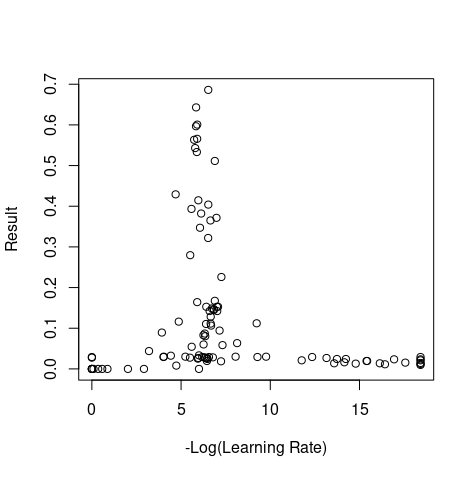
\includegraphics[scale=0.25]{hparams/plot-lr-reg.png}
    }
    \subfloat[LR, Categorization]{
        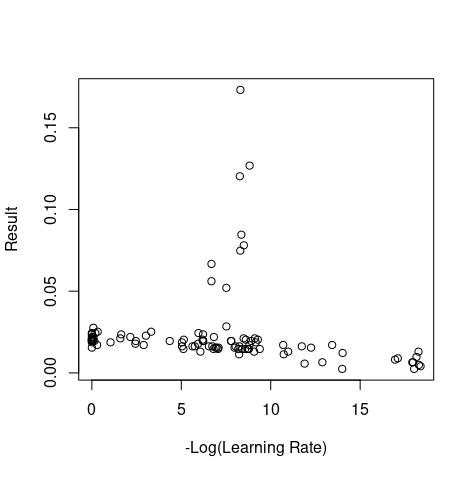
\includegraphics[scale=0.25]{hparams/plot-lr-cat.png}
    }
    \subfloat[Mechanism, Regression]{
        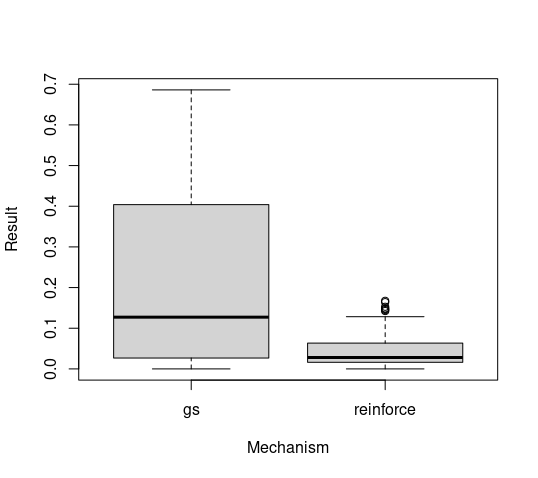
\includegraphics[scale=0.25]{hparams/boxplot-mech-reg.png}
    }
    \subfloat[Mechanism,\newline  Categorization]{
        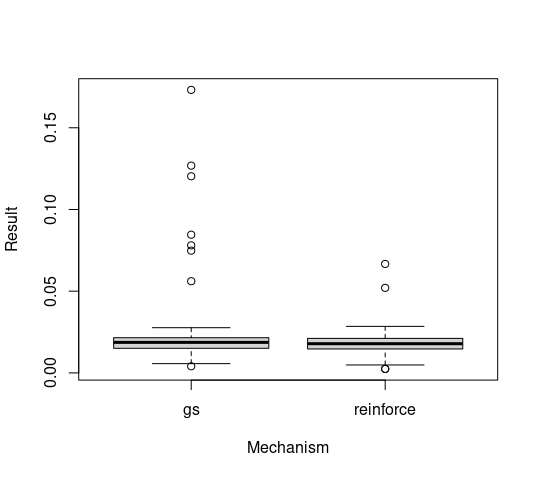
\includegraphics[scale=0.25]{hparams/boxplot-mech-cat.png}
    }
  
}

\makebox[0pt]{  
    \subfloat[Batch, Regression]{
        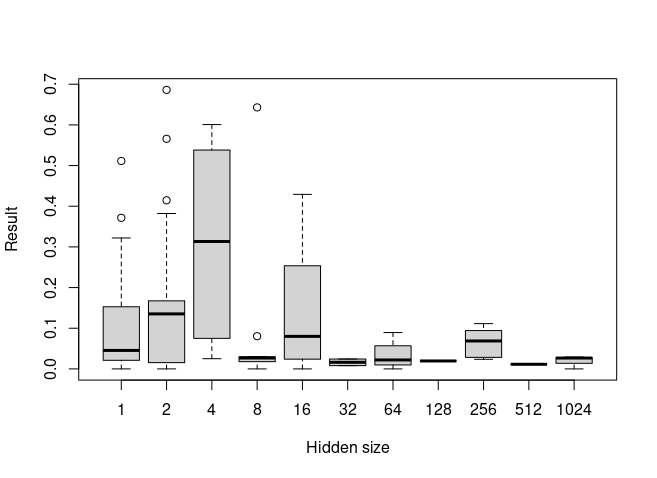
\includegraphics[scale=0.25]{hparams/boxplot-b-reg.png}
    }
    \subfloat[Batch, Categorization]{
        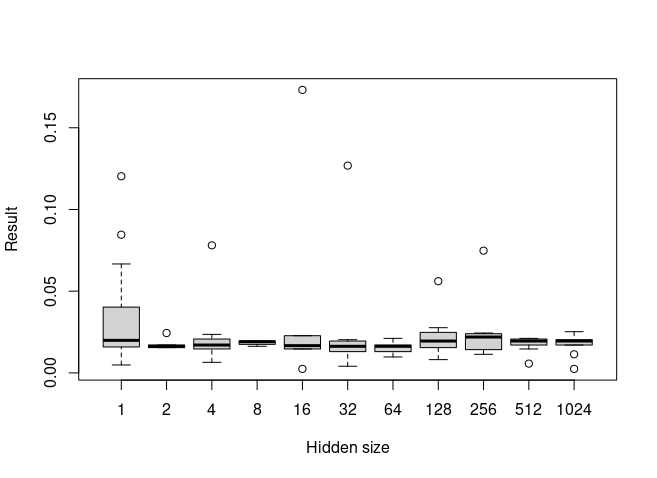
\includegraphics[scale=0.25]{hparams/boxplot-b-cat.png}
    }
    \subfloat[Loss aggregation,\newline Regression]{
        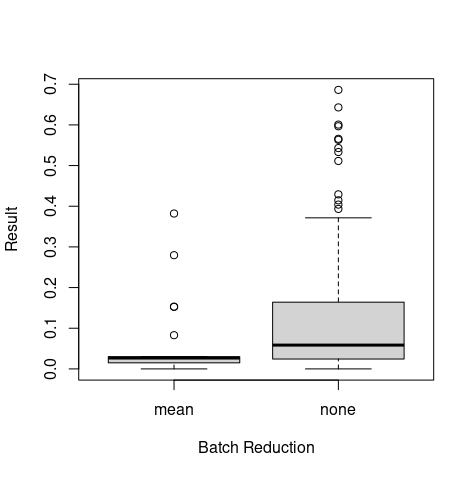
\includegraphics[scale=0.25]{hparams/boxplot-red-reg.png}
    }
    \subfloat[Loss aggregation,\newline Categorization]{
        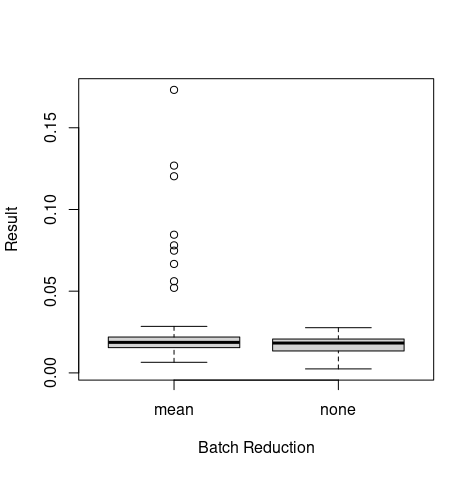
\includegraphics[scale=0.25]{hparams/boxplot-red-cat.png}
    }
}

\makebox[0pt]{  
    
    \subfloat[Input, Regression]{
        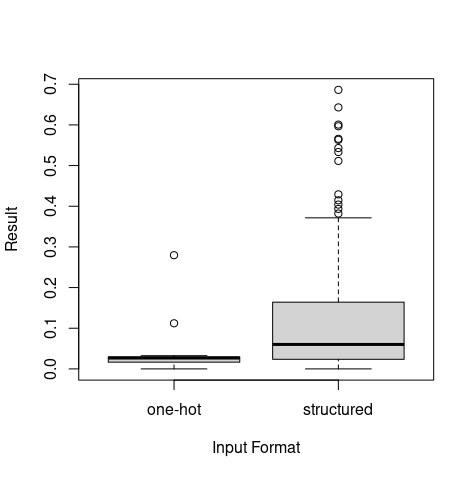
\includegraphics[scale=0.25]{hparams/boxplot-ipt-reg.png}
    }
    \subfloat[Input, Categorization]{
        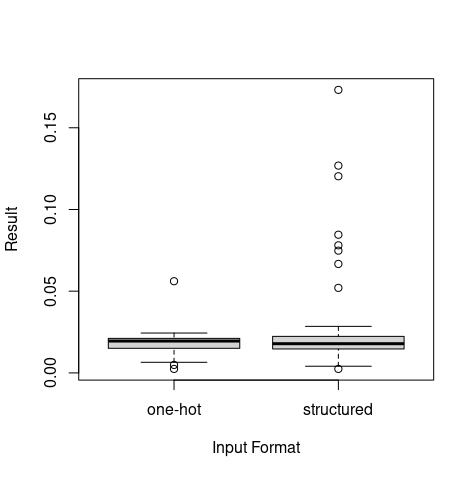
\includegraphics[scale=0.25]{hparams/boxplot-ipt-cat.png}
    }
    \subfloat[Hidden size, Regression]{
        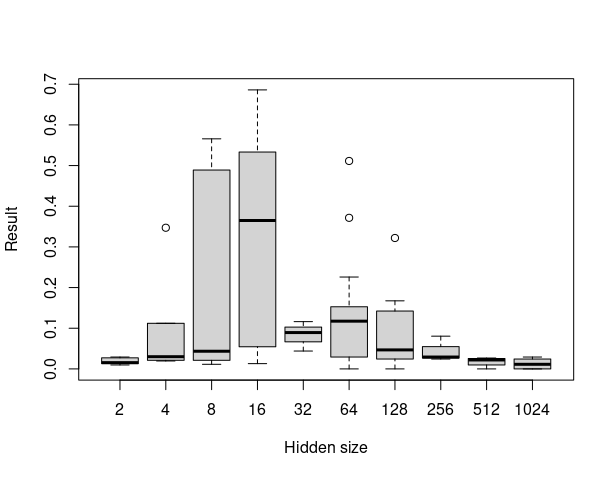
\includegraphics[scale=0.25]{hparams/boxplot-hid-reg.png}
    }
    \subfloat[Hidden size, Categorization]{
        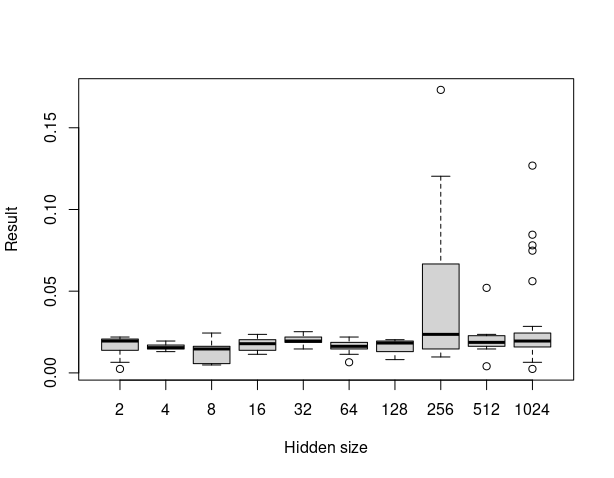
\includegraphics[scale=0.25]{hparams/boxplot-hid-cat.png}
    }
}

\makebox[0pt]{  
    
    \subfloat[Embedding size,\newline  Regression]{
        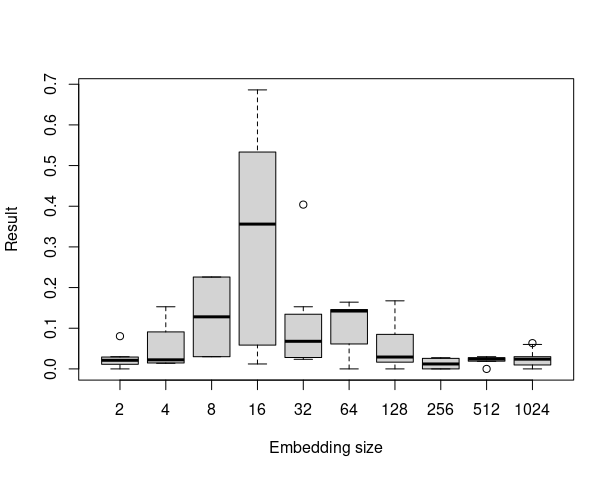
\includegraphics[scale=0.25]{hparams/boxplot-emb-reg.png}
    }
    \subfloat[Embedding size,\newline  Categorization]{
        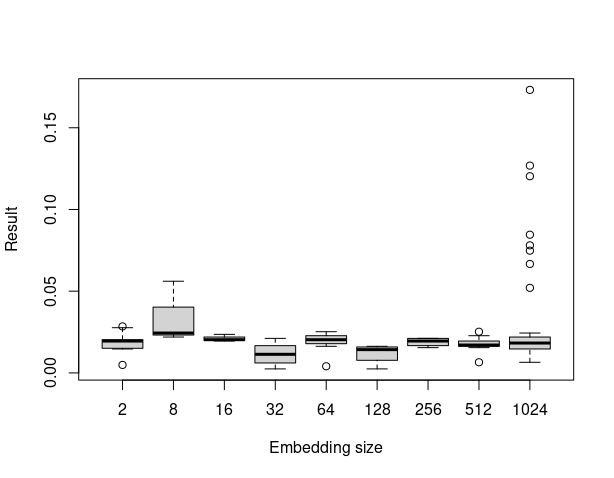
\includegraphics[scale=0.25]{hparams/boxplot-emb-cat.png}
    }
    \subfloat[Cell type,\newline  Regression]{
        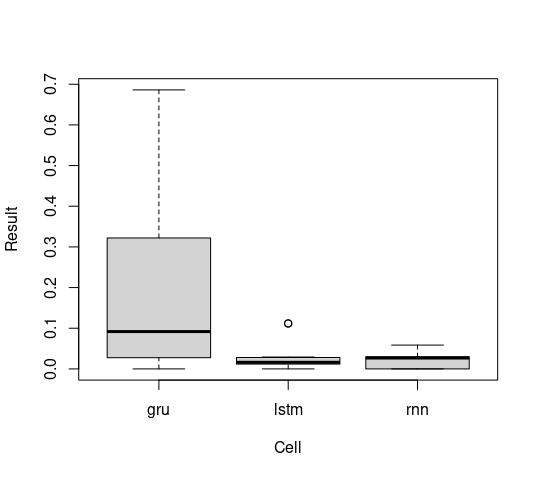
\includegraphics[scale=0.25]{hparams/boxplot-cell-reg.png}
    }
    \subfloat[Cell type,\newline  Categorization]{
        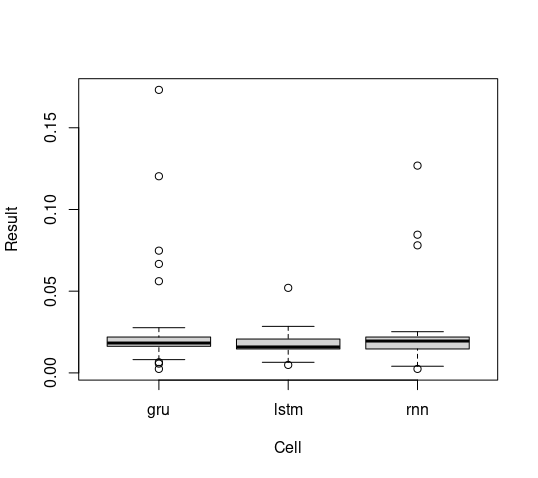
\includegraphics[scale=0.25]{hparams/boxplot-cell-cat.png}
    }
}

\makebox[0pt]{  
    
    \subfloat[Vocab size,\newline Regression]{
        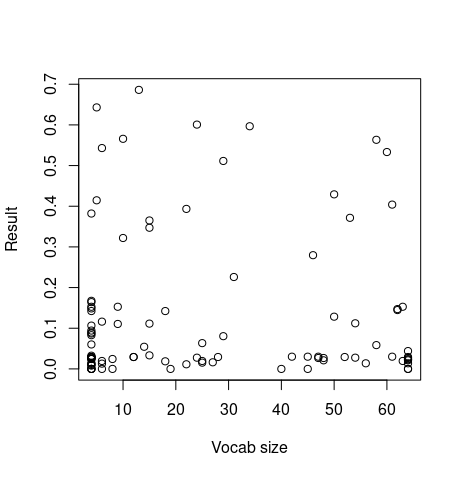
\includegraphics[scale=0.25]{hparams/plot-vocab-reg.png}
    }
    \subfloat[Vocab size,\newline Categorization]{
        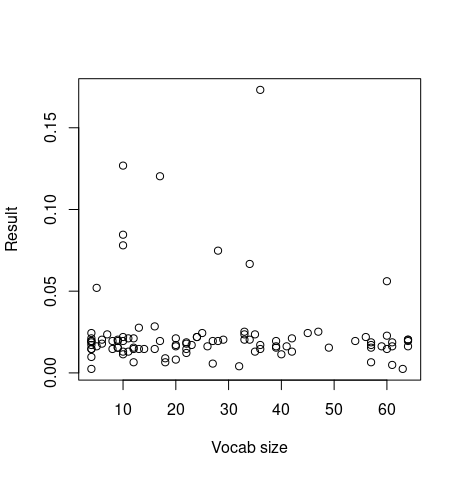
\includegraphics[scale=0.25]{hparams/plot-vocab-cat.png}
    }
    \subfloat[Curriculum,\newline  Regression]{
        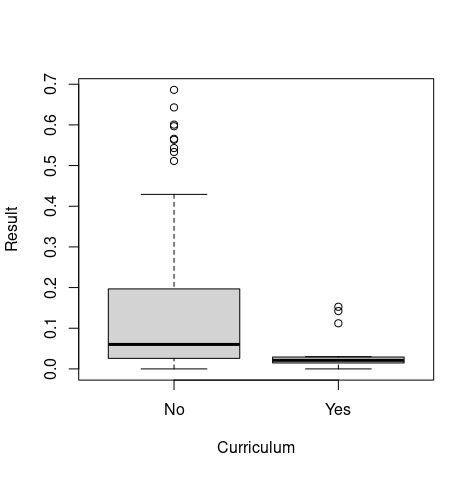
\includegraphics[scale=0.25]{hparams/boxplot-c-reg.png}
    }
    \subfloat[Curriculum,\newline  Categorization]{
        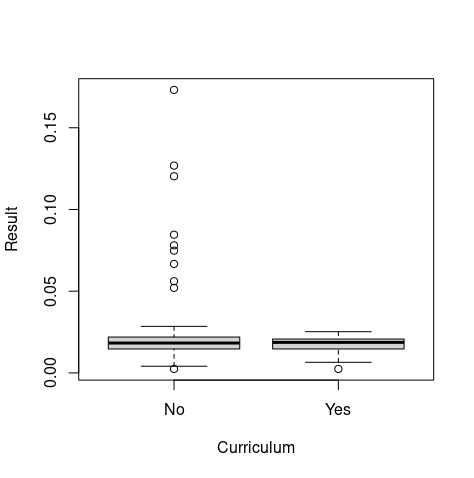
\includegraphics[scale=0.25]{hparams/boxplot-c-cat.png}
    }
}
    
    \caption{Overviews of hyperparameters sampled during selection process}
    \label{fig:hparams}
\end{figure*}
\end{document}
